% Created by tikzDevice version 0.12.6 on 2026-08-12 07:47:55
% !TEX encoding = UTF-8 Unicode
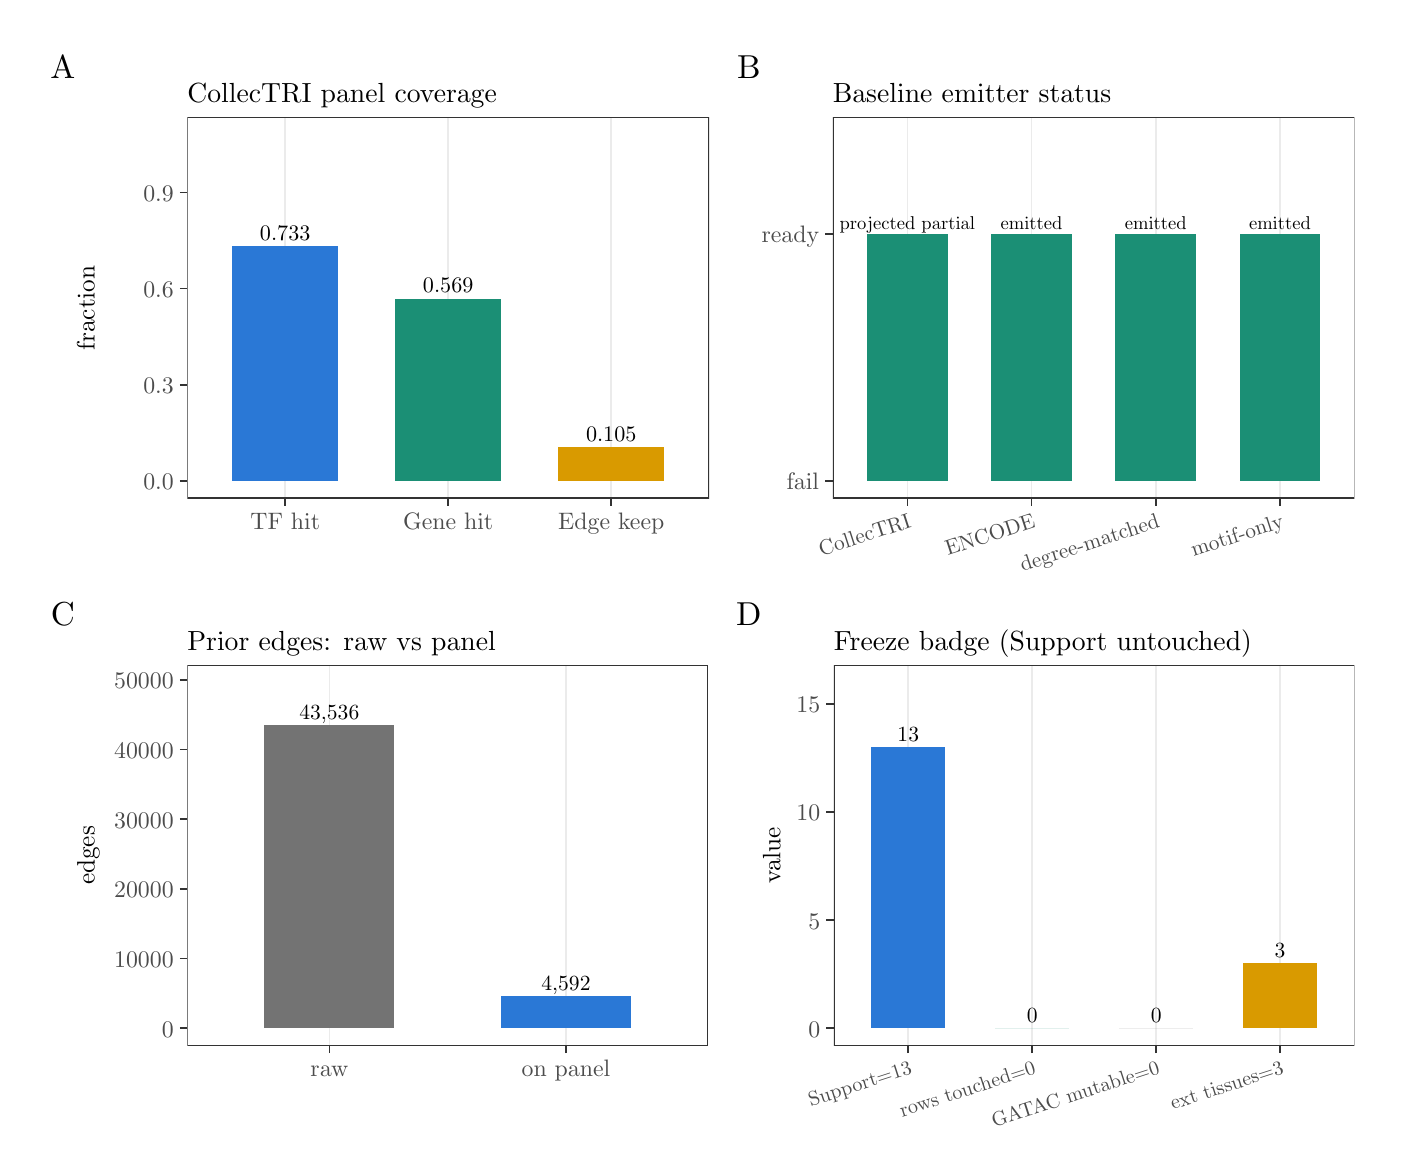
\begin{tikzpicture}[x=1pt,y=1pt]
\definecolor{fillColor}{RGB}{255,255,255}
\path[use as bounding box,fill=fillColor,fill opacity=0.00] (0,0) rectangle (491.44,404.71);
\begin{scope}
\path[clip] (  0.00,  0.00) rectangle (491.44,404.71);
\definecolor{drawColor}{RGB}{255,255,255}
\definecolor{fillColor}{RGB}{255,255,255}

\path[draw=drawColor,line width= 0.6pt,line join=round,line cap=round,fill=fillColor] ( -0.00,  0.00) rectangle (491.44,404.71);
\end{scope}
\begin{scope}
\path[clip] (  4.00,202.89) rectangle (252.22,400.71);
\definecolor{drawColor}{RGB}{255,255,255}
\definecolor{fillColor}{RGB}{255,255,255}

\path[draw=drawColor,line width= 0.6pt,line join=round,line cap=round,fill=fillColor] (  4.00,202.89) rectangle (252.22,400.71);
\end{scope}
\begin{scope}
\path[clip] (252.22,202.89) rectangle (485.44,400.71);
\definecolor{drawColor}{RGB}{255,255,255}
\definecolor{fillColor}{RGB}{255,255,255}

\path[draw=drawColor,line width= 0.6pt,line join=round,line cap=round,fill=fillColor] (252.22,202.89) rectangle (485.44,400.71);
\end{scope}
\begin{scope}
\path[clip] ( 57.71,234.70) rectangle (246.22,372.21);
\definecolor{fillColor}{RGB}{255,255,255}

\path[fill=fillColor] ( 57.71,234.70) rectangle (246.22,372.21);
\definecolor{drawColor}{gray}{0.92}

\path[draw=drawColor,line width= 0.6pt,line join=round] ( 93.06,234.70) --
	( 93.06,372.21);

\path[draw=drawColor,line width= 0.6pt,line join=round] (151.96,234.70) --
	(151.96,372.21);

\path[draw=drawColor,line width= 0.6pt,line join=round] (210.87,234.70) --
	(210.87,372.21);
\definecolor{fillColor}{RGB}{42,120,214}

\path[fill=fillColor] ( 73.91,240.95) rectangle (112.20,325.82);
\definecolor{fillColor}{RGB}{27,143,117}

\path[fill=fillColor] (132.82,240.95) rectangle (171.11,306.83);
\definecolor{fillColor}{RGB}{217,154,0}

\path[fill=fillColor] (191.73,240.95) rectangle (230.02,253.16);
\definecolor{drawColor}{RGB}{0,0,0}

\node[text=drawColor,anchor=base,inner sep=0pt, outer sep=0pt, scale=  0.80] at ( 93.06,327.90) {0.733};

\node[text=drawColor,anchor=base,inner sep=0pt, outer sep=0pt, scale=  0.80] at (151.96,308.91) {0.569};

\node[text=drawColor,anchor=base,inner sep=0pt, outer sep=0pt, scale=  0.80] at (210.87,255.24) {0.105};
\definecolor{drawColor}{gray}{0.20}

\path[draw=drawColor,line width= 0.6pt,line join=round,line cap=round] ( 57.71,234.70) rectangle (246.22,372.21);
\end{scope}
\begin{scope}
\path[clip] (  0.00,  0.00) rectangle (491.44,404.71);
\definecolor{drawColor}{gray}{0.30}

\node[text=drawColor,anchor=base east,inner sep=0pt, outer sep=0pt, scale=  0.86] at ( 52.76,237.76) {0.0};

\node[text=drawColor,anchor=base east,inner sep=0pt, outer sep=0pt, scale=  0.86] at ( 52.76,272.48) {0.3};

\node[text=drawColor,anchor=base east,inner sep=0pt, outer sep=0pt, scale=  0.86] at ( 52.76,307.21) {0.6};

\node[text=drawColor,anchor=base east,inner sep=0pt, outer sep=0pt, scale=  0.86] at ( 52.76,341.93) {0.9};
\end{scope}
\begin{scope}
\path[clip] (  0.00,  0.00) rectangle (491.44,404.71);
\definecolor{drawColor}{gray}{0.20}

\path[draw=drawColor,line width= 0.6pt,line join=round] ( 54.96,240.95) --
	( 57.71,240.95);

\path[draw=drawColor,line width= 0.6pt,line join=round] ( 54.96,275.68) --
	( 57.71,275.68);

\path[draw=drawColor,line width= 0.6pt,line join=round] ( 54.96,310.40) --
	( 57.71,310.40);

\path[draw=drawColor,line width= 0.6pt,line join=round] ( 54.96,345.13) --
	( 57.71,345.13);
\end{scope}
\begin{scope}
\path[clip] (  0.00,  0.00) rectangle (491.44,404.71);
\definecolor{drawColor}{gray}{0.20}

\path[draw=drawColor,line width= 0.6pt,line join=round] ( 93.06,231.95) --
	( 93.06,234.70);

\path[draw=drawColor,line width= 0.6pt,line join=round] (151.96,231.95) --
	(151.96,234.70);

\path[draw=drawColor,line width= 0.6pt,line join=round] (210.87,231.95) --
	(210.87,234.70);
\end{scope}
\begin{scope}
\path[clip] (  0.00,  0.00) rectangle (491.44,404.71);
\definecolor{drawColor}{gray}{0.30}

\node[text=drawColor,anchor=base,inner sep=0pt, outer sep=0pt, scale=  0.86] at ( 93.06,223.36) {TF hit};

\node[text=drawColor,anchor=base,inner sep=0pt, outer sep=0pt, scale=  0.86] at (151.96,223.36) {Gene hit};

\node[text=drawColor,anchor=base,inner sep=0pt, outer sep=0pt, scale=  0.86] at (210.87,223.36) {Edge keep};
\end{scope}
\begin{scope}
\path[clip] (  0.00,  0.00) rectangle (491.44,404.71);
\definecolor{drawColor}{RGB}{0,0,0}

\node[text=drawColor,rotate= 90.00,anchor=base,inner sep=0pt, outer sep=0pt, scale=  0.91] at ( 24.22,303.46) {fraction};
\end{scope}
\begin{scope}
\path[clip] (  0.00,  0.00) rectangle (491.44,404.71);
\definecolor{drawColor}{RGB}{0,0,0}

\node[text=drawColor,anchor=base west,inner sep=0pt, outer sep=0pt, scale=  1.00] at ( 57.71,377.58) {CollecTRI panel coverage};
\end{scope}
\begin{scope}
\path[clip] (  0.00,  0.00) rectangle (491.44,404.71);
\definecolor{drawColor}{RGB}{0,0,0}

\node[text=drawColor,anchor=base,inner sep=0pt, outer sep=0pt, scale=  1.20] at ( 12.74,386.41) {A};
\end{scope}
\begin{scope}
\path[clip] (290.93,234.70) rectangle (479.44,372.21);
\definecolor{fillColor}{RGB}{255,255,255}

\path[fill=fillColor] (290.93,234.70) rectangle (479.44,372.21);
\definecolor{drawColor}{gray}{0.92}

\path[draw=drawColor,line width= 0.6pt,line join=round] (317.86,234.70) --
	(317.86,372.21);

\path[draw=drawColor,line width= 0.6pt,line join=round] (362.74,234.70) --
	(362.74,372.21);

\path[draw=drawColor,line width= 0.6pt,line join=round] (407.63,234.70) --
	(407.63,372.21);

\path[draw=drawColor,line width= 0.6pt,line join=round] (452.51,234.70) --
	(452.51,372.21);
\definecolor{fillColor}{RGB}{27,143,117}

\path[fill=fillColor] (437.92,240.95) rectangle (467.09,330.25);

\path[fill=fillColor] (393.04,240.95) rectangle (422.21,330.25);

\path[fill=fillColor] (348.16,240.95) rectangle (377.33,330.25);

\path[fill=fillColor] (303.28,240.95) rectangle (332.45,330.25);
\definecolor{drawColor}{RGB}{0,0,0}

\node[text=drawColor,anchor=base,inner sep=0pt, outer sep=0pt, scale=  0.67] at (452.51,331.74) {emitted};

\node[text=drawColor,anchor=base,inner sep=0pt, outer sep=0pt, scale=  0.67] at (407.63,331.74) {emitted};

\node[text=drawColor,anchor=base,inner sep=0pt, outer sep=0pt, scale=  0.67] at (362.74,331.74) {emitted};

\node[text=drawColor,anchor=base,inner sep=0pt, outer sep=0pt, scale=  0.67] at (317.86,331.74) {projected partial};
\definecolor{drawColor}{gray}{0.20}

\path[draw=drawColor,line width= 0.6pt,line join=round,line cap=round] (290.93,234.70) rectangle (479.44,372.21);
\end{scope}
\begin{scope}
\path[clip] (  0.00,  0.00) rectangle (491.44,404.71);
\definecolor{drawColor}{gray}{0.30}

\node[text=drawColor,anchor=base east,inner sep=0pt, outer sep=0pt, scale=  0.86] at (285.98,237.76) {fail};

\node[text=drawColor,anchor=base east,inner sep=0pt, outer sep=0pt, scale=  0.86] at (285.98,327.05) {ready};
\end{scope}
\begin{scope}
\path[clip] (  0.00,  0.00) rectangle (491.44,404.71);
\definecolor{drawColor}{gray}{0.20}

\path[draw=drawColor,line width= 0.6pt,line join=round] (288.18,240.95) --
	(290.93,240.95);

\path[draw=drawColor,line width= 0.6pt,line join=round] (288.18,330.25) --
	(290.93,330.25);
\end{scope}
\begin{scope}
\path[clip] (  0.00,  0.00) rectangle (491.44,404.71);
\definecolor{drawColor}{gray}{0.20}

\path[draw=drawColor,line width= 0.6pt,line join=round] (317.86,231.95) --
	(317.86,234.70);

\path[draw=drawColor,line width= 0.6pt,line join=round] (362.74,231.95) --
	(362.74,234.70);

\path[draw=drawColor,line width= 0.6pt,line join=round] (407.63,231.95) --
	(407.63,234.70);

\path[draw=drawColor,line width= 0.6pt,line join=round] (452.51,231.95) --
	(452.51,234.70);
\end{scope}
\begin{scope}
\path[clip] (  0.00,  0.00) rectangle (491.44,404.71);
\definecolor{drawColor}{gray}{0.30}

\node[text=drawColor,rotate= 18.00,anchor=base east,inner sep=0pt, outer sep=0pt, scale=  0.77] at (319.63,224.31) {CollecTRI};

\node[text=drawColor,rotate= 18.00,anchor=base east,inner sep=0pt, outer sep=0pt, scale=  0.77] at (364.51,224.31) {ENCODE};

\node[text=drawColor,rotate= 18.00,anchor=base east,inner sep=0pt, outer sep=0pt, scale=  0.77] at (409.39,224.31) {degree-matched};

\node[text=drawColor,rotate= 18.00,anchor=base east,inner sep=0pt, outer sep=0pt, scale=  0.77] at (454.27,224.31) {motif-only};
\end{scope}
\begin{scope}
\path[clip] (  0.00,  0.00) rectangle (491.44,404.71);
\definecolor{drawColor}{RGB}{0,0,0}

\node[text=drawColor,anchor=base west,inner sep=0pt, outer sep=0pt, scale=  1.00] at (290.93,377.58) {Baseline emitter status};
\end{scope}
\begin{scope}
\path[clip] (  0.00,  0.00) rectangle (491.44,404.71);
\definecolor{drawColor}{RGB}{0,0,0}

\node[text=drawColor,anchor=base,inner sep=0pt, outer sep=0pt, scale=  1.20] at (260.60,386.41) {B};
\end{scope}
\begin{scope}
\path[clip] (  4.00,  3.00) rectangle (251.81,202.89);
\definecolor{drawColor}{RGB}{255,255,255}
\definecolor{fillColor}{RGB}{255,255,255}

\path[draw=drawColor,line width= 0.6pt,line join=round,line cap=round,fill=fillColor] (  4.00,  3.00) rectangle (251.81,202.89);
\end{scope}
\begin{scope}
\path[clip] (251.81,  3.00) rectangle (485.44,202.89);
\definecolor{drawColor}{RGB}{255,255,255}
\definecolor{fillColor}{RGB}{255,255,255}

\path[draw=drawColor,line width= 0.6pt,line join=round,line cap=round,fill=fillColor] (251.81,  3.00) rectangle (485.44,202.89);
\end{scope}
\begin{scope}
\path[clip] ( 57.71, 36.88) rectangle (245.81,174.39);
\definecolor{fillColor}{RGB}{255,255,255}

\path[fill=fillColor] ( 57.71, 36.88) rectangle (245.81,174.39);
\definecolor{drawColor}{gray}{0.92}

\path[draw=drawColor,line width= 0.6pt,line join=round] (109.01, 36.88) --
	(109.01,174.39);

\path[draw=drawColor,line width= 0.6pt,line join=round] (194.51, 36.88) --
	(194.51,174.39);
\definecolor{fillColor}{gray}{0.45}

\path[fill=fillColor] ( 85.50, 43.13) rectangle (132.52,152.79);
\definecolor{fillColor}{RGB}{42,120,214}

\path[fill=fillColor] (171.00, 43.13) rectangle (218.02, 54.70);
\definecolor{drawColor}{RGB}{0,0,0}

\node[text=drawColor,anchor=base,inner sep=0pt, outer sep=0pt, scale=  0.78] at (109.01,154.80) {43,536};

\node[text=drawColor,anchor=base,inner sep=0pt, outer sep=0pt, scale=  0.78] at (194.51, 56.71) { 4,592};
\definecolor{drawColor}{gray}{0.20}

\path[draw=drawColor,line width= 0.6pt,line join=round,line cap=round] ( 57.71, 36.88) rectangle (245.81,174.39);
\end{scope}
\begin{scope}
\path[clip] (  0.00,  0.00) rectangle (491.44,404.71);
\definecolor{drawColor}{gray}{0.30}

\node[text=drawColor,anchor=base east,inner sep=0pt, outer sep=0pt, scale=  0.86] at ( 52.76, 39.93) {0};

\node[text=drawColor,anchor=base east,inner sep=0pt, outer sep=0pt, scale=  0.86] at ( 52.76, 65.12) {10000};

\node[text=drawColor,anchor=base east,inner sep=0pt, outer sep=0pt, scale=  0.86] at ( 52.76, 90.31) {20000};

\node[text=drawColor,anchor=base east,inner sep=0pt, outer sep=0pt, scale=  0.86] at ( 52.76,115.50) {30000};

\node[text=drawColor,anchor=base east,inner sep=0pt, outer sep=0pt, scale=  0.86] at ( 52.76,140.68) {40000};

\node[text=drawColor,anchor=base east,inner sep=0pt, outer sep=0pt, scale=  0.86] at ( 52.76,165.87) {50000};
\end{scope}
\begin{scope}
\path[clip] (  0.00,  0.00) rectangle (491.44,404.71);
\definecolor{drawColor}{gray}{0.20}

\path[draw=drawColor,line width= 0.6pt,line join=round] ( 54.96, 43.13) --
	( 57.71, 43.13);

\path[draw=drawColor,line width= 0.6pt,line join=round] ( 54.96, 68.32) --
	( 57.71, 68.32);

\path[draw=drawColor,line width= 0.6pt,line join=round] ( 54.96, 93.51) --
	( 57.71, 93.51);

\path[draw=drawColor,line width= 0.6pt,line join=round] ( 54.96,118.69) --
	( 57.71,118.69);

\path[draw=drawColor,line width= 0.6pt,line join=round] ( 54.96,143.88) --
	( 57.71,143.88);

\path[draw=drawColor,line width= 0.6pt,line join=round] ( 54.96,169.07) --
	( 57.71,169.07);
\end{scope}
\begin{scope}
\path[clip] (  0.00,  0.00) rectangle (491.44,404.71);
\definecolor{drawColor}{gray}{0.20}

\path[draw=drawColor,line width= 0.6pt,line join=round] (109.01, 34.13) --
	(109.01, 36.88);

\path[draw=drawColor,line width= 0.6pt,line join=round] (194.51, 34.13) --
	(194.51, 36.88);
\end{scope}
\begin{scope}
\path[clip] (  0.00,  0.00) rectangle (491.44,404.71);
\definecolor{drawColor}{gray}{0.30}

\node[text=drawColor,anchor=base,inner sep=0pt, outer sep=0pt, scale=  0.86] at (109.01, 25.54) {raw};

\node[text=drawColor,anchor=base,inner sep=0pt, outer sep=0pt, scale=  0.86] at (194.51, 25.54) {on panel};
\end{scope}
\begin{scope}
\path[clip] (  0.00,  0.00) rectangle (491.44,404.71);
\definecolor{drawColor}{RGB}{0,0,0}

\node[text=drawColor,rotate= 90.00,anchor=base,inner sep=0pt, outer sep=0pt, scale=  0.91] at ( 24.22,105.63) {edges};
\end{scope}
\begin{scope}
\path[clip] (  0.00,  0.00) rectangle (491.44,404.71);
\definecolor{drawColor}{RGB}{0,0,0}

\node[text=drawColor,anchor=base west,inner sep=0pt, outer sep=0pt, scale=  1.00] at ( 57.71,179.76) {Prior edges: raw vs panel};
\end{scope}
\begin{scope}
\path[clip] (  0.00,  0.00) rectangle (491.44,404.71);
\definecolor{drawColor}{RGB}{0,0,0}

\node[text=drawColor,anchor=base,inner sep=0pt, outer sep=0pt, scale=  1.20] at ( 12.74,188.58) {C};
\end{scope}
\begin{scope}
\path[clip] (291.34, 36.88) rectangle (479.44,174.39);
\definecolor{fillColor}{RGB}{255,255,255}

\path[fill=fillColor] (291.34, 36.88) rectangle (479.44,174.39);
\definecolor{drawColor}{gray}{0.92}

\path[draw=drawColor,line width= 0.6pt,line join=round] (318.21, 36.88) --
	(318.21,174.39);

\path[draw=drawColor,line width= 0.6pt,line join=round] (362.99, 36.88) --
	(362.99,174.39);

\path[draw=drawColor,line width= 0.6pt,line join=round] (407.78, 36.88) --
	(407.78,174.39);

\path[draw=drawColor,line width= 0.6pt,line join=round] (452.56, 36.88) --
	(452.56,174.39);
\definecolor{fillColor}{RGB}{42,120,214}

\path[fill=fillColor] (304.77, 43.13) rectangle (331.64,144.70);
\definecolor{fillColor}{RGB}{27,143,117}

\path[fill=fillColor] (349.56, 43.13) rectangle (376.43, 43.13);
\definecolor{fillColor}{gray}{0.45}

\path[fill=fillColor] (394.34, 43.13) rectangle (421.22, 43.13);
\definecolor{fillColor}{RGB}{217,154,0}

\path[fill=fillColor] (439.13, 43.13) rectangle (466.00, 66.57);
\definecolor{drawColor}{RGB}{0,0,0}

\node[text=drawColor,anchor=base,inner sep=0pt, outer sep=0pt, scale=  0.78] at (318.21,146.71) {13};

\node[text=drawColor,anchor=base,inner sep=0pt, outer sep=0pt, scale=  0.78] at (362.99, 45.14) {0};

\node[text=drawColor,anchor=base,inner sep=0pt, outer sep=0pt, scale=  0.78] at (407.78, 45.14) {0};

\node[text=drawColor,anchor=base,inner sep=0pt, outer sep=0pt, scale=  0.78] at (452.56, 68.58) {3};
\definecolor{drawColor}{gray}{0.20}

\path[draw=drawColor,line width= 0.6pt,line join=round,line cap=round] (291.34, 36.88) rectangle (479.44,174.39);
\end{scope}
\begin{scope}
\path[clip] (  0.00,  0.00) rectangle (491.44,404.71);
\definecolor{drawColor}{gray}{0.30}

\node[text=drawColor,anchor=base east,inner sep=0pt, outer sep=0pt, scale=  0.86] at (286.39, 39.93) {0};

\node[text=drawColor,anchor=base east,inner sep=0pt, outer sep=0pt, scale=  0.86] at (286.39, 79.00) {5};

\node[text=drawColor,anchor=base east,inner sep=0pt, outer sep=0pt, scale=  0.86] at (286.39,118.06) {10};

\node[text=drawColor,anchor=base east,inner sep=0pt, outer sep=0pt, scale=  0.86] at (286.39,157.13) {15};
\end{scope}
\begin{scope}
\path[clip] (  0.00,  0.00) rectangle (491.44,404.71);
\definecolor{drawColor}{gray}{0.20}

\path[draw=drawColor,line width= 0.6pt,line join=round] (288.59, 43.13) --
	(291.34, 43.13);

\path[draw=drawColor,line width= 0.6pt,line join=round] (288.59, 82.20) --
	(291.34, 82.20);

\path[draw=drawColor,line width= 0.6pt,line join=round] (288.59,121.26) --
	(291.34,121.26);

\path[draw=drawColor,line width= 0.6pt,line join=round] (288.59,160.32) --
	(291.34,160.32);
\end{scope}
\begin{scope}
\path[clip] (  0.00,  0.00) rectangle (491.44,404.71);
\definecolor{drawColor}{gray}{0.20}

\path[draw=drawColor,line width= 0.6pt,line join=round] (318.21, 34.13) --
	(318.21, 36.88);

\path[draw=drawColor,line width= 0.6pt,line join=round] (362.99, 34.13) --
	(362.99, 36.88);

\path[draw=drawColor,line width= 0.6pt,line join=round] (407.78, 34.13) --
	(407.78, 36.88);

\path[draw=drawColor,line width= 0.6pt,line join=round] (452.56, 34.13) --
	(452.56, 36.88);
\end{scope}
\begin{scope}
\path[clip] (  0.00,  0.00) rectangle (491.44,404.71);
\definecolor{drawColor}{gray}{0.30}

\node[text=drawColor,rotate= 18.00,anchor=base east,inner sep=0pt, outer sep=0pt, scale=  0.73] at (319.87, 26.81) {Support=13};

\node[text=drawColor,rotate= 18.00,anchor=base east,inner sep=0pt, outer sep=0pt, scale=  0.73] at (364.66, 26.81) {rows touched=0};

\node[text=drawColor,rotate= 18.00,anchor=base east,inner sep=0pt, outer sep=0pt, scale=  0.73] at (409.44, 26.81) {GATAC mutable=0};

\node[text=drawColor,rotate= 18.00,anchor=base east,inner sep=0pt, outer sep=0pt, scale=  0.73] at (454.23, 26.81) {ext tissues=3};
\end{scope}
\begin{scope}
\path[clip] (  0.00,  0.00) rectangle (491.44,404.71);
\definecolor{drawColor}{RGB}{0,0,0}

\node[text=drawColor,rotate= 90.00,anchor=base,inner sep=0pt, outer sep=0pt, scale=  0.91] at (272.03,105.63) {value};
\end{scope}
\begin{scope}
\path[clip] (  0.00,  0.00) rectangle (491.44,404.71);
\definecolor{drawColor}{RGB}{0,0,0}

\node[text=drawColor,anchor=base west,inner sep=0pt, outer sep=0pt, scale=  1.00] at (291.34,179.76) {Freeze badge (Support untouched)};
\end{scope}
\begin{scope}
\path[clip] (  0.00,  0.00) rectangle (491.44,404.71);
\definecolor{drawColor}{RGB}{0,0,0}

\node[text=drawColor,anchor=base,inner sep=0pt, outer sep=0pt, scale=  1.20] at (260.55,188.58) {D};
\end{scope}
\end{tikzpicture}
